% !Mode:: "TeX:UTF-8"
% Translator: Yujun Li 
\chapter{实践方法论}
\label{chap:practical_methodology}
要成功地使用深度学习技术,仅仅知道存在哪些算法和解释他们为何有效的原理是不够的。
一个优秀的机器学习实践者还需要知道如何针对具体应用挑选一个合适的算法以及如何监控,并根据实验反馈改进机器学习系统。
在\gls{ML}系统的日常开发中,实践者需要决定是否收集更多的数据、增加或减少模型\gls{capacity}、添加或删除\gls{regularization}项、改进模型的优化、改进模型的近似推断或调试模型的软件实现。
尝试这些操作都需要大量时间,因此确定正确做法,而不盲目猜测尤为重要的。


本书的大部分内容都是关于不同的\gls{ML}模型、训练算法和\gls{objective_function}。
这可能给人一种印象——成为\gls{ML}专家的最重要因素是了解各种各样的\gls{ML}技术,并熟悉各种不同的数学。
在实践中,正确使用一个普通算法通常比草率地使用一个不清楚的算法效果更好。
正确应用一个算法需要掌握一些相当简单的方法论。
本章的许多建议都来自\cite{ng-lecture-advice}。


我们建议参考以下几个实践设计流程:
\begin{itemize}
\item 确定目标——使用什么样的\gls{error_metric},并为此\gls{error_metric}指定目标值。
这些目标和\gls{error_metric}取决于该应用旨在解决的问题。
% -- 409 end


\item 尽快建立一个\gls{end_to_end}的工作流程,包括估计合适的\gls{performance_metrics}。
% 410 head

\item 搭建系统,并确定性能瓶颈。
检查哪个部分的性能差于预期,以及是否是因为\gls{overfitting}、\gls{underfitting},或者数据或软件缺陷造成的。

\item 根据具体观察反复地进行增量式的改动,如收集新数据、调整\gls{hyperparameter}或改进算法。
\end{itemize}


我们将使用街景地址号码\gls{transcription_system}\citep{Goodfellow+et+al-ICLR2014a}作为一个运行示例。
该应用的目标是将建筑物添加到谷歌地图。
街景车拍摄建筑物,并记录与每张建筑照片相关的GPS坐标。
\gls{convolutional_network}识别每张照片上的地址号码,由谷歌地图数据库在正确的位置添加该地址。
这个商业应用是一个很好的示例,它的开发流程遵循我们倡导的设计方法。

% 410 mid
我们现在描述这个过程中的每一个步骤。



\section{\glsentrytext{performance_metrics}}
\label{sec:performance_metrics}
确定目标,即使用什么\gls{error_metric},是必要的第一步,因为\gls{error_metric}将指导接下来的所有工作。
同时我们也应该了解大概能得到什么级别的目标性能。
% 410 mid


值得注意的是对于大多数应用而言,不可能实现绝对零误差。
即使你有无限的训练数据,并且恢复了真正的\gls{PD},\gls{bayes_error}仍定义了能达到的最小\gls{error_rate}。
这是因为输入特征可能无法包含输出变量的完整信息,或是因为系统可能本质上是随机的。
当然我们还会受限于有限的训练数据。

% 410 end
训练数据的数量会因为各种原因受到限制。
当目标是打造现实世界中最好的产品或服务时,我们通常需要收集更多的数据,但必须确定进一步减少误差的价值,并与收集更多数据的成本做权衡。
数据收集会耗费时间、金钱,或带来人体痛苦(例如,收集人体医疗测试数据)。
科研中,目标通常是在某个确定\gls{benchmarks}下探讨哪个算法更好,一般会固定\gls{training_set},不允许收集更多的数据。
% 411 head


如何确定合理的性能期望?
在学术界,通常我们可以根据先前公布的\gls{benchmarks}结果来估计预期\gls{error_rate}。
在现实世界中,一个应用的\gls{error_rate}有必要是安全的、具有成本效益的或吸引消费者的。
一旦你确定了想要达到的\gls{error_rate},那么你的设计将由如何达到这个\gls{error_rate}来指导。
% 411 mid


除了需要考虑\gls{performance_metrics}之外,另一个需要考虑的是度量的选择。
我们有几种不同的\gls{performance_metrics},可以用来度量一个含有\gls{ML}组件的完整应用的有效性。
这些\gls{performance_metrics}通常不同于训练模型的\gls{cost_function}。 
如\secref{sec:the_performance_measure_p}所述,我们通常会度量一个系统的\gls{accuracy},或等价地,\gls{error_rate}。


然而,许多应用需要更高级的度量。
% 411 mid

有时,一种错误可能会比另一种错误更严重。
例如,垃圾邮件检测系统会有两种错误:将正常邮件错误地归为垃圾邮件,将垃圾邮件错误地归为正常邮件。
阻止正常消息比允许可疑消息通过糟糕得多。
我们希望度量某种形式的总\gls{cost},其中拦截正常邮件比允许垃圾邮件通过的\gls{cost}更高,而不是度量垃圾邮件分类的\gls{error_rate}。
% 411 mid


有时,我们需要训练检测某些罕见事件的二元分类器。
例如,我们可能会为一种罕见疾病设计医疗测试。
假设每一百万人中只有一人患病。
我们只需要让分类器一直报告没有患者,就能轻易地在检测任务上实现$99.9999\%$的正确率。
显然,正确率很难描述这种系统的性能。
解决这个问题的方法是度量\firstgls{precision}和\firstgls{recall}。
\gls{precision}是模型报告的检测是正确的比率,而\gls{recall}则是真实事件被检测到的比率。
检测器永远报告没有患者,会得到一个完美的\gls{precision},但\gls{recall}为零。
而报告每个人都是患者的检测器会得到一个完美的\gls{recall},但是\gls{precision}会等于人群中患有该病的比例(在我们的例子是$0.0001\%$,每一百万人只有一人患病)。
当使用\gls{precision}和\gls{recall}时,我们通常会画\firstgls{prcurve},$y$轴表示\gls{precision},$x$轴表示\gls{recall}。
如果检测到的事件发生了,那么分类器会返回一个较高的得分。
例如,我们将\gls{feedforward_network}设计为检测一种疾病,估计一个医疗结果由特征$\Vx$表示的人患病的概率为$\hat{y} = P(y=1\mid\Vx)$。
每当这个得分超过某个阈值时,我们报告检测结果。
通过调整阈值,我们能权衡\gls{precision}和\gls{recall}。
在很多情况下,我们希望用一个数而不是曲线来概括分类器的性能。
要做到这一点,我们可以将\gls{precision} $p$和\gls{recall} $r$转换为\firstgls{fscore}
\begin{equation}
	F = \frac{2pr}{p+r}.
\end{equation}
另一种方法是报告\gls{prcurve}下方的总面积。
% -- 412 head


在一些应用中,\gls{ML}系统可能会拒绝做出判断。
如果\gls{ML}算法能够估计所作判断的置信度,这将会非常有用,特别是在错误判断会导致严重危害,而人工操作员能够偶尔接管的情况下。
街景\gls{transcription_system}可以作为这种情况的一个示例。
这个任务是识别照片上的地址号码,将照片拍摄地点对应到地图上的地址。%??  翻译的很有问题
如果地图是不精确的,那么地图的价值会严重下降。
因此只在转录正确的情况下添加地址十分重要。
如果\gls{ML}系统认为它不太能像人一样正确地转录,那么最好办法当然是让人来转录照片。
当然,只有当\gls{ML}系统能够大量降低需要人工操作处理的图片时,它才是有用的。
在这种情况下,一种自然的\gls{performance_measures}是\firstgls{coverage}。
\gls{coverage}是\gls{ML}系统能够产生响应的样本所占的比率。
我们权衡\gls{coverage}和\gls{precision}。
一个系统可以通过拒绝处理任意样本的方式来达到$100\%$的\gls{precision},但是\gls{coverage}降到了$0\%$。
对于街景任务,该项目的目标是达到人类级别的转录\gls{precision},同时保持$95\%$的\gls{coverage}。
在这项任务中,人类级别的性能是$98\%$的\gls{precision}。
% 412 end

还有许多其他的\gls{performance_measures}。
例如,我们可以度量点击率、收集用户满意度调查等等。
许多专业的应用领域也有特定的标准。
% 412 end

最重要的是首先要确定改进哪个\gls{performance_measures},然后专心提高\gls{performance_measures}。
如果没有明确的目标,那么我们很难判断\gls{ML}系统上的改动是否有所改进。

% -- 412 end

\section{默认的\glsentrytext{baseline}模型}
\label{sec:default_baseline_models}
确定\gls{performance_metrics}和目标后,任何实际应用的下一步是尽快建立一个合理的\gls{end_to_end}系统。
本节给出了一些关于在不同情况下使用哪种算法作为第一个\gls{baseline}方法推荐。
在本节中,我们提供了关于不同情况下使用哪种算法作为第一\gls{baseline}方法的推荐。
值得注意的是,\gls{DL}研究进展迅速,所以本书出版后很快可能会有更好的默认算法。
% 413 head 

根据问题的复杂性,项目开始时可能无需使用\gls{DL}。
如果只需正确地选择几个线性权重就可能解决问题,那么项目可以开始于一个简单的统计模型,如\gls{logistic_regression}。


如果问题属于``\glssymbol{AI}-完全''类的,如\gls{object_recognition}、\gls{SR}、\gls{machine_translation}等等,那么项目开始于一个合适的\gls{DL}模型,效果会比较好。
% 413 mid 


首先,根据数据的结构选择一类合适的模型。
如果项目是以固定大小的向量作为输入的\gls{supervised_learning},那么可以使用全连接的\gls{feedforward_network}。
如果输入有已知的拓扑结构(例如,输入是图像),那么可以使用\gls{convolutional_network}。
在这些情况下,刚开始可以使用某些\gls{piecewise}线性单元(\glssymbol{ReLU}或者其扩展,如\glssymbol{leaky_ReLU}、\glssymbol{PReLU}和\glssymbol{maxout})。
如果输入或输出是一个序列,可以使用\gls{gated_recurrent_net}(\glssymbol{LSTM}或\glssymbol{gated_recurrent_unit})。
% 413 mid 

具有衰减\gls{learning_rate}以及\gls{momentum}的\glssymbol{SGD}是优化算法一个合理的选择
(流行的衰减方法有,衰减到固定最低\gls{learning_rate}的线性衰减、指数衰减,或每次发生验证错误停滞时将\gls{learning_rate}降低$2-10$倍,这些衰减方法在不同问题上好坏不一)。
另一个非常合理的选择是Adam算法。
\gls{batch_normalization}对优化性能有着显著的影响,特别是对\gls{convolutional_network}和具有\gls{sigmoid}非线性函数的网络而言。
虽然在最初的\gls{baseline}中忽略\gls{batch_normalization}是合理的,然而当优化似乎出现问题时,应该立刻使用\gls{batch_normalization}。
% 413 mid 


除非\gls{training_set}包含数千万以及更多的样本,否则项目应该在一开始就包含一些温和的\gls{regularization}。 
\gls{early_stopping}也被普遍采用。
\gls{dropout}也是一个很容易实现,且兼容很多模型和训练算法的出色\gls{regularizer}。
\gls{batch_normalization}有时也能降低\gls{generalization_error},此时可以省略\gls{dropout}步骤,因为用于标准化变量的统计量估计本身就存在\gls{noise}。 %?? 还是有问题
% -- 413 --  end


如果我们的任务和另一个被广泛研究的任务相似,那么通过复制先前研究中已知性能良好的模型和算法,可能会得到很好的效果。
甚至可以从该任务中复制一个训练好的模型。
例如,通常会使用在ImageNet上训练好的\gls{convolutional_network}的特征来解决其他\gls{CV}任务\citep{girshickregion}。
% 414 head


一个常见问题是项目开始时是否使用\gls{unsupervised_learning},我们将在第三部分进一步探讨这个问题。
 这个问题和特定领域有关。
在某些领域,比如\gls{NLP},能够大大受益于\gls{unsupervised_learning}技术,如学习\gls{unsupervised}\gls{word_embeddings}。
在其他领域,如\gls{CV},除非是在\gls{semi_supervised}的设定下(\gls{labeled}样本数量很少)\citep{Kingma-et-al-NIPS2014,Rasmus-et-al-arxiv2015},目前\gls{unsupervised_learning}并没有带来益处。
如果应用所在环境中,\gls{unsupervised_learning}被认为是很重要的,那么将其包含在第一个\gls{end_to_end}\gls{baseline}中。
否则,只有在解决\gls{unsupervised}问题时,才会第一次尝试时使用\gls{unsupervised_learning}。
在发现初始\gls{baseline}\gls{overfitting}的时候,我们可以尝试加入\gls{unsupervised_learning}。
% 414 mid


\section{决定是否收集更多数据}
\label{sec:determining_whether_to_gather_more_data}

在建立第一个\gls{end_to_end}系统后,就可以度量算法性能并决定如何改进算法。
许多\gls{ML}新手都忍不住尝试很多不同的算法来进行改进。
然而,收集更多的数据往往比改进学习算法要有用得多。
% 414 mid


怎样判断是否要收集更多的数据?
首先,确定\gls{training_set}上的性能是否可接受。
如果模型在\gls{training_set}上的性能就很差,学习算法都不能在\gls{training_set}上学习出良好的模型,那么就没必要收集更多的数据。
反之,可以尝试增加更多的网络层或每层增加更多的\gls{hidden_unit},以增加模型的规模。
此外,也可以尝试调整\gls{learning_rate}等\gls{hyperparameter}的措施来改进学习算法。
如果更大的模型和仔细调试的优化算法效果不佳,那么问题可能源自训练数据的\emph{质量}。
数据可能含太多\gls{noise},或是可能不包含预测输出所需的正确输入。
这意味着我们需要重新开始,收集更干净的数据或是收集特征更丰富的数据集。
% -- 414 end


如果\gls{training_set}上的性能是可接受的,那么我们开始度量\gls{test_set}上的性能。
如果\gls{test_set}上的性能也是可以接受的,那么就顺利完成了。
如果\gls{test_set}上的性能比\gls{training_set}的要差得多,那么收集更多的数据是最有效的解决方案之一。
这时主要的考虑是收集更多数据的代价和可行性,其他方法降低\gls{test_error}的代价和可行性,和增加数据数量能否显著提升\gls{test_set}性能。
在拥有百万甚至上亿用户的大型网络公司,收集大型数据集是可行的,并且这样做的成本可能比其他方法要少很多,所以答案几乎总是收集更多的训练数据。
例如,收集大型\gls{labeled}数据集是解决\gls{object_recognition}问题的主要因素之一。
在其他情况下,如医疗应用,收集更多的数据可能代价很高或者不可行。
一个可以替代的简单方法是降低模型大小或是改进\gls{regularization}(调整\gls{hyperparameter},如\gls{weight_decay}系数,或是加入\gls{regularization}策略,如\gls{dropout})。
如果调整\gls{regularization}\gls{hyperparameter}后,\gls{training_set}性能和\gls{test_set}性能之间的差距还是不可接受,那么收集更多的数据是可取的。
% 415 mid


在决定是否收集更多的数据时,也需要确定收集多少数据。
如\figref{fig:chap5_training_size_grows}所示,绘制曲线显示\gls{training_set}规模和\gls{generalization_error}之间的关系是很有帮助的。
根据走势延伸曲线,可以预测还需要多少训练数据来达到一定的性能。
通常,加入总数目一小部分的样本不会对\gls{generalization_error}产生显著的影响。
因此,建议在对数尺度上考虑\gls{training_set}的大小,例如在后续的实验中倍增样本数目。
% 415 mid


如果收集更多的数据是不可行的,那么改进\gls{generalization_error}的唯一方法是改进学习算法本身。
这属于研究领域,并非对应用实践者的建议。

\section{选择\glsentrytext{hyperparameter}}
\label{sec:selecting_hyperparameters}
大部分\gls{DL}算法都有许多\gls{hyperparameter}来控制不同方面的算法表现。
有些\gls{hyperparameter}会影响算法运行的时间和存储成本。
有些\gls{hyperparameter}会影响学习到的模型质量,以及在新输入上推断正确结果的能力。
% -- 415 -end


有两种选择\gls{hyperparameter}的基本方法:手动选择和自动选择。
手动选择\gls{hyperparameter}需要了解\gls{hyperparameter}做了些什么,以及\gls{ML}模型如何才能取得良好的\gls{generalization}。
自动选择\gls{hyperparameter}算法大大减少了解这些想法的需要,但它们往往需要更高的计算成本。
% 416 head


\subsection{手动调整\glsentrytext{hyperparameter}}
\label{sec:manual_hyperparameter_tuning}
手动设置\gls{hyperparameter},我们必须了解\gls{hyperparameter}、\gls{training_error}、\gls{generalization_error}和计算资源(内存和运行时间)之间的关系。
这需要切实了解一个学习算法有效\gls{capacity}的基础概念,如\chapref{chap:machine_learning_basics}所描述的。
% 416 mid


手动搜索\gls{hyperparameter}的目标通常是最小化受限于运行时间和内存预算的\gls{generalization_error}。
我们不去探讨如何确定各种\gls{hyperparameter}对运行时间和内存的影响,因为这高度依赖于平台。


手动搜索\gls{hyperparameter}的主要目标是调整模型的有效\gls{capacity}以匹配任务的复杂性。
有效\gls{capacity}受限于三个因素:模型的表示\gls{capacity}、学习算法成功最小化训练模型\gls{cost_function}的能力以及\gls{cost_function}和训练过程\gls{regularize}模型的程度。
具有更多网络层,每层有更多\gls{hidden_unit}的模型具有较高的表示能力——能够表示更复杂的函数。
然而,如果训练算法不能找到某个合适的函数来最小化训练\gls{cost},或是\gls{regularization}项(如\gls{weight_decay})排除了这些合适的函数,那么即使模型的表达能力较高,也不能学习出合适的函数。%??  还是太乱

% 416 mid


当\gls{generalization_error}以某个\gls{hyperparameter}为变量,作为函数绘制出来时,通常会表现为U形曲线,如\figref{fig:chap5_generalization_vs_capacity}所示。
在某个极端情况下,\gls{hyperparameter}对应着低\gls{capacity},并且\gls{generalization_error}由于\gls{training_error}较大而很高。
这便是\gls{underfitting}的情况。
另一种极端情况,\gls{hyperparameter}对应着高\gls{capacity},并且\gls{generalization_error}由于\gls{training_error}和\gls{test_error}之间的差距较大而很高。
最优的模型\gls{capacity}位于曲线中间的某个位置,能够达到最低可能的\gls{generalization_error},由某个中等的\gls{generalization_error}和某个中等的\gls{training_error}相加构成。
% -- 416 end



对于某些\gls{hyperparameter},当\gls{hyperparameter}数值太大时,会发生\gls{overfitting}。
例如中间层\gls{hidden_unit}的数量,增加数量能提高模型的\gls{capacity},容易发生\gls{overfitting}。%??  原文不符 
对于某些\gls{hyperparameter},当\gls{hyperparameter}数值太小时,也会发生\gls{overfitting}。
例如,最小的\gls{weight_decay}系数允许为零,此时学习算法具有最大的有效\gls{capacity},反而容易\gls{overfitting}。%??  原文不符   这一段好像偏差较大 
% 417 head


并非每个\gls{hyperparameter}都能对应着完整的U形曲线。
很多\gls{hyperparameter}是离散的,如中间层单元数目或是\gls{maxout_unit}中线性元件的数目,这种情况只能沿曲线探索一些点。
有些\gls{hyperparameter}是二值的。
通常这些\gls{hyperparameter}用来指定是否使用学习算法中的一些可选部分,如预处理步骤减去均值并除以标准差来标准化输入特征。
这些\gls{hyperparameter}只能探索曲线上的两点。
其他一些\gls{hyperparameter}可能会有最小值或最大值,限制其探索曲线的某些部分。%??    
例如,\gls{weight_decay}系数最小是零。
这意味着,如果\gls{weight_decay}系数为零时模型\gls{underfitting},那么我们将无法通过修改\gls{weight_decay}系数探索\gls{overfitting}区域。
换言之,有些\gls{hyperparameter}只能减少模型\gls{capacity}。
% 417 mid


\gls{learning_rate}可能是最重要的\gls{hyperparameter}。
如果你只有时间调整一个\gls{hyperparameter},那就调整\gls{learning_rate}。
相比其他\gls{hyperparameter},它以一种更复杂的方式控制模型的有效\gls{capacity}——当\gls{learning_rate}适合优化问题时,模型的有效\gls{capacity}最高,此时\gls{learning_rate}是\emph{正确}的,既不是特别大也不是特别小。
\gls{learning_rate}关于\emph{\gls{training_error}}具有U形曲线,如\figref{fig:chap11_lr}所示。
当\gls{learning_rate}过大时,\gls{GD}可能会不经意地增加而非减少\gls{training_error}。
在理想化的二次情况下,如果\gls{learning_rate}是最佳值的两倍大时,会发生这种情况\citep{LeCun+98backprop-small}。
当\gls{learning_rate}太小,训练不仅慢,还有可能永久停留在一个很高的\gls{training_error}。
关于这种效应,我们知之甚少(不会发生于一个凸\gls{loss_function}中)。
% 417 end

\begin{figure}[!htb]
\ifOpenSource
\centerline{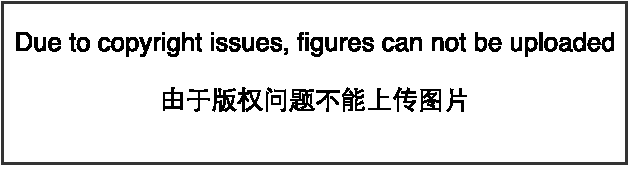
\includegraphics{figure.pdf}}
\else
\centerline{\includegraphics{Chapter11/figures/lr_color}}
\fi
\caption{\gls{training_error}和\gls{learning_rate}之间的典型关系。
注意当\gls{learning_rate}大于最优值时误差会有显著的提升。
此图针对固定的训练时间,越小的\gls{learning_rate}有时候可以以一个正比于\gls{learning_rate}减小量的因素来减慢训练过程。
\gls{generalization_error}也会得到类似的曲线,由于正则项作用在\gls{learning_rate}过大或过小处比较复杂。
由于一个糟糕的优化从某种程度上说可以避免\gls{overfitting},即使是\gls{training_error}相同的点也会拥有完全不同的\gls{generalization_error}。}
\label{fig:chap11_lr}
\end{figure}

% 417 end
调整\gls{learning_rate}外的其他参数时,需要同时监测\gls{training_error}和\gls{test_error},以判断模型是否\gls{overfitting}或\gls{underfitting},然后适当调整其\gls{capacity}。


如果\gls{training_set}错误率大于目标\gls{error_rate},那么只能增加模型\gls{capacity}以改进模型。
如果没有使用\gls{regularization},并且确信优化算法正确运行,那么有必要添加更多的网络层或\gls{hidden_unit}。
然而,令人遗憾的是,这增加了模型的计算代价。
% 418 head


如果\gls{test_set}错误率大于目标\gls{error_rate},那么可以采取两个方法。
\gls{test_error}是\gls{training_error}和\gls{test_error}之间差距与\gls{training_error}的总和。
寻找最佳的\gls{test_error}需要权衡这些数值。
当\gls{training_error}较小(因此\gls{capacity}较大),\gls{test_error}主要取决于\gls{training_error}和\gls{test_error}之间的差距时,通常神经网络效果最好。
此时目标是缩小这一差距,使\gls{training_error}的增长速率不快于差距减小的速率。
要减少这个差距,我们可以改变\gls{regularization}\gls{hyperparameter},以减少有效的模型\gls{capacity},如添加\gls{dropout}或\gls{weight_decay}策略。
通常,最佳性能来自\gls{regularization}得很好的大规模模型,比如使用\gls{dropout}的神经网络。
% 418 mid


大部分\gls{hyperparameter}可以通过推理其是否增加或减少模型\gls{capacity}来设置。
部分示例如表\ref{tab:hyperparameter_effect}所示。


% 418 end
手动调整\gls{hyperparameter}时,不要忘记最终目标:提升\gls{test_set}性能。
加入\gls{regularization}只是实现这个目标的一种方法。
只要\gls{training_error}低,随时都可以通过收集更多的训练数据来减少\gls{generalization_error}。
实践中能够确保学习有效的的暴力方法就是不断提高模型\gls{capacity}和\gls{training_set}的大小,直到解决问题。
这种做法增加了训练和推断的计算代价,所以只有在拥有足够资源时才是可行的。
原则上,这种做法可能会因为优化难度提高而失败,但对于许多问题而言,优化似乎并没有成为一个显著的障碍,当然,前提是选择了合适的模型。
% 419 end


% -- 419
\begin{table}
\centering
\small
\begin{tabular}{p{2.5cm}|p{1.5cm}|p{4.0cm}|p{4.0cm}}
\gls{hyperparameter} & \gls{capacity}何时增加 & 原因  & 注意事项 \\
\hline
\gls{hidden_unit}数量 &  增加          & 增加\gls{hidden_unit}数量会增加模型的\gls{representation}能力。 & 几乎模型每个操作所需的时间和内存代价都会随\gls{hidden_unit}数量的增加而增加。\\
\hline
\gls{learning_rate} & 调至最优 & 不正确的学习速率,不管是太高还是太低都会由于优化失败而导致低有效\gls{capacity}的模型。
 & \\
\hline
卷积核宽度 & 增加 & 增加卷积核宽度会增加模型的参数数量。&
较宽的卷积核导致较窄的输出尺寸,除非使用隐式零填充减少此影响,否则会降低模型\gls{capacity}。 
较宽的卷积核需要更多的内存存储参数,并会增加运行时间,但较窄的输出会降低内存代价。
\\
\hline
隐式零填充 & 增加 & 在卷积之前隐式添加零能保持较大尺寸的\gls{representation}。&
大多数操作的时间和内存代价会增加。\\
\hline
\gls{weight_decay}系数 & 降低 & 降低\gls{weight_decay}系数使得模型参数可以自由地变大。
 & \\
\hline
\gls{dropout}比率 & 降低 & 较少地丢弃单元可以更多地让单元彼此``协力''来适应\gls{training_set}。
 & \\
\end{tabular}
\caption{各种\gls{hyperparameter}对模型\gls{capacity}的影响。}
\label{tab:hyperparameter_effect}
\index{Dropout}
\index{Weight decay}
\end{table}
% -- 419




\subsection{自动\glsentrytext{hyperparameter}优化算法}
\label{sec:automatic_hyperparameter_optimization_algorithms}
理想的学习算法应该是只需要输入一个数据集,就可以输出学习的函数,而不需要手动调整\gls{hyperparameter}。
一些流行的学习算法,如\gls{logistic_regression}和\gls{SVM},流行的部分原因是这类算法只有一到两个\gls{hyperparameter}需要调整,它们也能表现出不错的性能。
有些情况下,所需调整的\gls{hyperparameter}数量较少时,神经网络可以表现出不错的性能;但\gls{hyperparameter}数量有几十甚至更多时,效果会提升得更加明显。
当使用者有一个很好的初始值,例如由在相同类型的应用和架构上具有经验的人确定初始值,或者使用者在相似问题上具有几个月甚至几年的神经网络\gls{hyperparameter}调整经验,那么手动调整\gls{hyperparameter}能有很好的效果。%??  由在相同类型的应用和架构上具有经验的人确定初始  这句话好像不对吧? --没觉得有问题,你觉得是什么了
然而,对于很多应用而言,这些起点都不可用。
在这些情况下,自动算法可以找到合适的\gls{hyperparameter}。
% 420 head


如果我们仔细想想使用者搜索学习算法合适\gls{hyperparameter}的方式,我们会意识到这其实是一种优化:
我们在试图寻找\gls{hyperparameter}来优化\gls{objective_function},例如验证误差,有时还会有一些约束(如训练时间,内存或识别时间的预算)。
因此,原则上有可能开发出封装学习算法的\firstgls{hyperparameter_optimization}算法,并选择其\gls{hyperparameter},从而使用者不需要指定学习算法的\gls{hyperparameter}。
令人遗憾的是,\gls{hyperparameter}优化算法往往有自己的\gls{hyperparameter},如学习算法的每个\gls{hyperparameter}应该被探索的值的范围。
然而,这些次级\gls{hyperparameter}通常很容易选择,这是说,相同的次级\gls{hyperparameter}能够很多不同的问题上具有良好的性能。
% 420 mid


\subsection{\glsentrytext{grid_search}}
\label{sec:grid_search}
当有三个或更少的\gls{hyperparameter}时,常见的\gls{hyperparameter}搜索方法是\firstgls{grid_search}。
对于每个\gls{hyperparameter},使用者选择一个较小的有限值集去探索。
然后,这些\gls{hyperparameter}笛卡尔乘积得到一组组\gls{hyperparameter},\gls{grid_search}使用每组\gls{hyperparameter}训练模型。
挑选\gls{validation_set}误差最小的\gls{hyperparameter}作为最好的\gls{hyperparameter}。
如\figref{fig:chap11_grid_vs_random}所示\gls{hyperparameter}值的网络。
% -- 420 end


\begin{figure}[!htb]
\ifOpenSource
\centerline{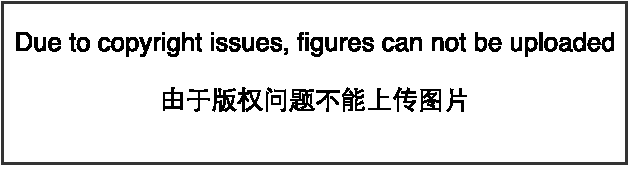
\includegraphics{figure.pdf}}
\else
\begin{tabular}{cc}
\includegraphics[width=0.4\textwidth]{Chapter11/figures/grid} &
\includegraphics[width=0.4\textwidth]{Chapter11/figures/random}
\end{tabular}
\fi
\caption{\gls{grid_search}和\gls{random_search}的比较。
为了方便地说明,我们只展示两个\gls{hyperparameter}的例子,但是我们关注的问题中\gls{hyperparameter}个数通常会更多。
\emph{(左)}为了实现\gls{grid_search},我们为每个\gls{hyperparameter}提供了一个值的集合。
搜索算法对每一种在这些集合的交叉积中的\gls{hyperparameter}组合进行训练。
\emph{(右)}为了实现\gls{random_search},我们给联合\gls{hyperparameter}赋予了一个概率分布。
通常\gls{hyperparameter}之间是相互独立的。
常见的这种分布的选择是均匀分布或者是对数均匀(从对数均匀分布中抽样,就是对从均匀分布中抽取的样本进行指数运算)的。
然后这些搜索算法从联合的\gls{hyperparameter}空间中采样,然后运行每一个样本。
\gls{grid_search}和\gls{random_search}都运行了\gls{validation_set}上的误差并返回了最优的解。
这个图说明了通常只有一个\gls{hyperparameter}对结果有着重要的影响。
在这个例子中,只有水平轴上的\gls{hyperparameter}对结果有重要的作用。
\gls{grid_search}将大量的计算浪费在了指数量级的对结果无影响的\gls{hyperparameter}中,相比之下\gls{random_search}几乎每次测试都测试了对结果有影响的每个\gls{hyperparameter}的独一无二的值。
此图经\citet{Bergstra+Bengio-LW2011}允许转载。}
\label{fig:chap11_grid_vs_random}
\end{figure}


应该如何选择搜索集合的范围呢?
在\gls{hyperparameter}是数值(有序)的情况下,每个列表的最小和最大的元素可以基于先前相似实验的经验保守地挑选出来,以确保最优解非常可能在所选范围内。
通常,\gls{grid_search}大约会在\firstgls{logarithmic_scale}下挑选合适的值,例如,一个\gls{learning_rate}的取值集合是$\{0.1,0.01,10^{-3},10^{-4},10^{-5}\}$,或者\gls{hidden_unit}数目的取值集合$\{50,100,200,500,1000,2000\}$。
% 421 head


通常重复进行\gls{grid_search}时,效果会最好。
例如,假设我们在集合$\{-1,0,1\}$上\gls{grid_search}\gls{hyperparameter} $\alpha$。
如果找到的最佳值是$1$,那么说明我们低估了最优值$\alpha$所在的范围,应该改变搜索格点,例如在集合$\{1,2,3\}$中搜索。
如果最佳值是$0$,那么我们不妨通过细化搜索范围以改进估计,在集合$\{-0.1,0,0.1\}$上进行\gls{grid_search}。
% -- 422 head


\gls{grid_search}带来的一个明显问题是,计算代价会随着\gls{hyperparameter}数量呈指数级增长。
如果有$m$个\gls{hyperparameter},每个最多取$n$个值,那么训练和估计所需的试验数将是$O(n^m)$。
我们可以并行地进行实验,并且并行要求十分宽松(进行不同搜索的机器之间几乎没有必要进行通信)。
令人遗憾的是,由于\gls{grid_search}指数级增长计算代价,即使是并行,我们也无法提供令人满意的搜索规模。


\subsection{\glsentrytext{random_search}}
\label{sec:random_search}
幸运的是,有一个替代\gls{grid_search}的方法,并且编程简单,使用更方便,能更快地收敛到\gls{hyperparameter}的良好取值:\gls{random_search}\citep{Bergstra+Bengio-2012-small}。
% 422


\gls{random_search}过程如下。
首先,我们为每个\gls{hyperparameter}定义一个边缘分布,例如,\gls{bernoulli_distribution}或\gls{categorical_distribution}(分别对应着二元\gls{hyperparameter}或离散\gls{hyperparameter}),或者\gls{logarithmic_scale}上的均匀分布(对应着正实值\gls{hyperparameter})。
例如,
\begin{align}
	\texttt{log\_learning\_rate} &\sim u(-1, -5), \\
	\texttt{learning\_rate} &= 10^{\texttt{log\_learning\_rate}},
\end{align}
其中,$u(a,b)$表示区间$(a,b)$上均匀采样的样本。
类似地,$\texttt{log\_number\_of\_hidden\_units}$可以从$u(\log(50), \log(2000))$上采样。
% 422 mid


与\gls{grid_search}不同,我们\emph{不需要离散化}\gls{hyperparameter}的值。这允许我们在一个更大的集合上进行搜索,而不产生额外的计算代价。%?? bin 不知道如何翻译bin,你有什么好的翻译没 
实际上,如\figref{fig:chap11_grid_vs_random}所示,当有几个\gls{hyperparameter}对\gls{performance_metrics}没有显著影响时,\gls{random_search}相比于\gls{grid_search}指数级地高效。
\cite{Bergstra+Bengio-2012-small}进行了详细的研究并发现相比于\gls{grid_search}, \gls{random_search}能够更快地减小\gls{validation_set}误差(就每个模型运行的试验数而言)。
% 422 end

与\gls{grid_search}一样,我们通常会重复运行不同版本的\gls{random_search},以基于前一次运行的结果改进下一次搜索。
% 422 end


\gls{random_search}能比\gls{grid_search}更快地找到良好\gls{hyperparameter}的原因是,没有浪费的实验,不像\gls{grid_search}有时会对一个\gls{hyperparameter}的两个不同值(给定其他\gls{hyperparameter}值不变)给出相同结果。
在\gls{grid_search}中,其他\gls{hyperparameter}将在这两次实验中拥有相同的值,而在\gls{random_search}中,它们通常会具有不同的值。
因此,如果这两个值的变化所对应的\gls{validation_set}误差没有明显区别的话,\gls{grid_search}没有必要重复两个等价的实验,而\gls{random_search}仍然会对其他\gls{hyperparameter}进行两次独立地探索。

% 423 head

\subsection{基于模型的\glsentrytext{hyperparameter}优化}
\label{sec:model_based_hyperparameter_optimization}
\gls{hyperparameter}搜索问题可以转化为一个优化问题。
决策变量是\gls{hyperparameter}。
优化的\gls{cost}是\gls{hyperparameter}训练出来的模型在\gls{validation_set}上的误差。
在简化的设定下,可以计算\gls{validation_set}上可导误差函数关于\gls{hyperparameter}的梯度,然后我们遵循这个梯度更新\citep{bengio:1999:snowbird,bengio-hyper-NC00,maclaurin2015gradient}。
令人遗憾的是,在大多数实际设定中,这个梯度是不可用的。
这可能是因为其高额的计算代价和存储成本,也可能是因为\gls{validation_set}误差在\gls{hyperparameter}上本质上不可导,例如\gls{hyperparameter}是离散值的情况。
% 423 mid


为了弥补梯度的缺失,我们可以对\gls{validation_set}误差建模,然后通过优化该模型来提出新的\gls{hyperparameter}猜想。
大部分基于模型的\gls{hyperparameter}搜索算法,都是使用贝叶斯回归模型来估计每个\gls{hyperparameter}的\gls{validation_set}误差期望和该期望的不确定性。
因此,优化涉及到探索(探索高度不确定的\gls{hyperparameter},可能带来显著的效果提升,也可能效果很差)和使用(使用已经确信效果不错的\gls{hyperparameter}——通常是先前见过的非常熟悉的\gls{hyperparameter})之间的权衡。
关于\gls{hyperparameter}优化的最前沿方法还包括Spearmint\citep{Snoek+al-NIPS2012-small},TPE\citep{Bergstra+al-NIPS2011}和SMAC\citep{hutter+hoos+leyton+brown:2011}。


% 423 end
目前,我们无法明确确定,贝叶斯\gls{hyperparameter}优化是否是一个能够实现更好\gls{DL}结果或是能够事半功倍的成熟工具。
贝叶斯\gls{hyperparameter}优化有时表现得像人类专家,能够在有些问题上取得很好的效果,但有时又会在某些问题上发生灾难性的失误。
看看它是否适用于一个特定的问题是值得尝试的,但目前该方法还不够成熟或可靠。
就像所说的那样,\gls{hyperparameter}优化是一个重要的研究领域,通常主要受\gls{DL}所需驱动,但是它不仅能贡献于整个\gls{ML}领域,还能贡献于一般的工程学。
% 424 head


大部分\gls{hyperparameter}优化算法比\gls{random_search}更复杂,并且具有一个共同的缺点,在它们能够从实验中提取任何信息之前,它们需要运行完整的训练实验。
相比于人类实践者手动搜索,考虑实验早期可以收集的信息量,这种方法是相当低效的,因为手动搜索通常可以很早判断出某组\gls{hyperparameter}是否是完全病态的。
\cite{swersky2014freeze}提出了一个可以维护多个实验的早期版本算法。
在不同的时间点,\gls{hyperparameter}优化算法可以选择开启一个新实验,``冻结''正在运行但希望不大的实验,或是``解冻''并恢复早期被冻结的,但现在根据更多信息后又有希望的实验。


% 424
\section{调试策略}
\label{sec:debugging_strategies}
当一个\gls{ML}系统效果不好时,通常很难判断效果不好的原因是算法本身,还是算法实现错误。
由于各种原因,\gls{ML}系统很难调试。


% 424
在大多数情况下,我们不能提前知道算法的行为。
事实上,使用\gls{ML}的整个出发点是,它会发现一些我们自己无法发现的有用行为。
如果我们在一个\emph{新}的分类任务上训练一个神经网络,它达到$5\%$的\gls{test_error},我们没法直接知道这是期望的结果,还是次优的结果。


另一个难点是,大部分\gls{ML}模型有多个自适应的部分。
如果一个部分失效了,其他部分仍然可以自适应,并获得大致可接受的性能。
例如,假设我们正在训练多层神经网络,其中参数为权重$\MW$和\gls{bias_aff} $\Vb$。
进一步假设,我们单独手动实现了每个参数的\gls{GD}规则。
而我们在偏置更新时犯了一个错误:
\begin{equation}
	\Vb \leftarrow \Vb - \alpha,
\end{equation}
其中$\alpha$是\gls{learning_rate}。
这个错误更新没有使用梯度。
它会导致偏置在整个学习中不断变为负值,对于一个学习算法来说这显然是错误的。 
然而只是检查模型输出的话,该错误可能并不是显而易见的。
根据输入的分布,权重可能可以自适应地补偿负的偏置。
% -- 425 head


大部分神经网络的调试策略都是解决这两个难题的一个或两个。
我们可以设计一种足够简单的情况,能够提前得到正确结果,判断模型预测是否与之相符;我们也可以设计一个测试,独立检查神经网络实现的各个部分。


一些重要的调试检测如下所列。

\emph{可视化计算中模型的行为}:%??  in action 
当训练模型检测图像中的对象时,查看一些模型检测到部分重叠的图像。
在训练语音生成模型时,试听一些生成的语音样本。
这似乎是显而易见的,但在实际中很容易只注意量化\gls{performance_metrics},如\gls{accuracy}或对数似然。
直接观察\gls{ML}模型运行其任务,有助于确定其达到的量化性能数据是否看上去合理。
错误评估模型性能可能是最具破坏性的错误之一,因为它们会使你在系统出问题时误以为系统运行良好。
% 425 mid


\emph{可视化最严重的错误}:
大多数模型能够输出运行任务时的某种置信度量。
例如,基于\gls{softmax}输出层的分类器给每个类分配一个概率。
因此,分配给最有可能的类的概率给出了模型在其分类决定上的置信估计值。
通常,相比于正确预测的概率最大似然训练会略有高估。
但是由于实际上模型的较小概率不太可能对应着正确的标签,因此它们在一定意义上还是有些用的。
通过查看\gls{training_set}中很难正确建模的样本,通常可以发现该数据预处理或者标记方式的问题。
例如,街景\gls{transcription_system}原本有个问题是,地址号码检测系统会将图像裁剪得过于紧密,而省略掉了一些数字。
然后转录网络会给这些图像的正确答案分配非常低的概率。
将图像排序,确定置信度最高的错误,显示系统的裁剪有问题。
修改检测系统裁剪更宽的图像,从而使整个系统获得更好的性能,但是转录网络需要能够处理地址号码中位置和范围更大变化的情况。
% 425 end


\emph{根据训练和\gls{test_error}检测软件}:
我们往往很难确定底层软件是否是正确实现。
训练和\gls{test_error}能够提供一些线索。
如果\gls{training_error}较低,但是\gls{test_error}较高,那么很有可能训练过程是在正常运行,但模型由于算法原因\gls{overfitting}了。
另一种可能是,\gls{test_error}没有被正确地度量,可能是由于训练后保存模型再重载去度量\gls{test_set}时出现问题,或者是因为测试数据和训练数据预处理的方式不同。
如果训练和\gls{test_error}都很高,那么很难确定是软件错误,还是由于算法原因模型\gls{underfitting}。
这种情况需要进一步的测试,如下面所述。

% -- 426 head

\emph{拟合极小的数据集}:
当\gls{training_set}上有很大的误差时,我们需要确定问题是真正的\gls{underfitting},还是软件错误。
通常,即使是小模型也可以保证很好地拟合一个足够小的数据集。
例如,只有一个样本的分类数据可以通过正确设置输出层的偏置来拟合。
通常,如果不能训练一个分类器来正确标注一个单独的样本,或不能训练一个\gls{AE}来成功地精准再现一个单独的样本,或不能训练一个生成模型来一致地生成一个单独的样本,那么很有可能是由于软件错误阻止\gls{training_set}上的成功优化。
此测试可以扩展到只有少量样本的小数据集上。

% 426 mid

\emph{比较反向传播导数和数值导数}:
如果读者正在使用一个需要实现梯度计算的软件框架,或者在添加一个新操作到求导库中,必须定义它的\texttt{bprop}方法,那么常见的错误原因是没能正确地实现梯度表达。
验证这些求导正确性的一种方法是比较实现的自动求导和通过\firstgls{finite_difference}计算的导数。
因为
\begin{equation}
	f'(x) = \lim_{\epsilon \to 0} \frac{f(x+\epsilon) - f(x)}{\epsilon},
\end{equation}
我们可以使用小的、有限的$\epsilon$近似导数:
\begin{equation}
	f'(x) \approx \frac{f(x+\epsilon) - f(x)}{\epsilon}.
\end{equation}
我们可以使用\firstgls{centered_difference}提高近似的\gls{accuracy}:
\begin{equation}
	f'(x) \approx \frac{ f(x+\frac{1}{2}\epsilon) - f(x-\frac{1}{2}\epsilon) }{\epsilon}.
\end{equation}
扰动大小$\epsilon$必须足够大,以确保该扰动不会由于数值计算的有限\gls{precision}问题产生舍入误差。

% 426 end

通常,我们会测试向量值函数$g:\SetR^m \to \SetR^n$的梯度或\gls{jacobian}矩阵。
令人遗憾的是,\gls{finite_difference}只允许我们每次计算一个导数。
我们可以使用\gls{finite_difference} $mn$次评估$g$的所有偏导数,也可以将该测试应用于一个新函数(在函数$g$的输入输出都加上随机投影)。%??  后面这句好像不对?  g的输入输出都使用随机投影的
例如,我们可以将导数实现的测试用于函数$f(x) = \Vu^T g(\Vv x)$,其中$\Vu$和$\Vv$是随机向量。%??  这句也不对
正确计算$f'(x)$要求能够正确地通过$g$反向传播,但是使用\gls{finite_difference}能够高效地计算,因为$f$只有一个输入和一个输出。
通常,一个好的方法是在多个$\Vu$值和$\Vv$值上重复这个测试,可以减少测试忽略了垂直于随机投影的错误的几率。%??  很难

% 427 head

如果我们可以在复数上进行数值计算,那么使用复数作为函数的输入会有非常高效的数值方法估算梯度\citep{Squire+Trapp-1998}。
该方法基于如下观察
\begin{align}
	f(x + i\epsilon) &= f(x) + i\epsilon f'(x) + O(\epsilon^2) ,\\
	\text{real}( f(x+i\epsilon) ) &= f(x) + O(\epsilon^2), \quad \text{image}( \frac{f(x+i\epsilon)}{ \epsilon } ) = f'(x) + O(\epsilon^2),
\end{align}
其中$i=\sqrt{-1}$。
和上面的实值情况不同,这里不存在消除影响,因为我们对$f$在不同点上计算差分。
因此我们可以使用很小的$\epsilon$,比如$\epsilon = 10^{-150}$,其中误差$O(\epsilon^2)$对所有实用目标都是微不足道的。

% 427 mid

\emph{监控激活函数值和梯度的直方图}:
可视化神经网络在大量训练迭代后(也许是一个\gls{epoch})收集到的激活函数值和梯度的统计量往往是有用的。
\gls{hidden_unit}的预激活值可以告诉我们该单元是否饱和,或者它们饱和的频率如何。
例如,对于整流器,它们多久关一次?是否有单元一直关闭?
对于双曲正切单元而言,预激活绝对值的平均值可以告诉我们该单元的饱和程度。
在深度网络中,传播梯度的快速增长或快速消失,可能会阻碍优化过程。
最后,比较参数梯度和参数的量级也是有帮助的。
正如\citep{Bottou-DLSS2015}所建议的,我们希望参数在一个\gls{minibatch}更新中变化的幅度是参数量值$1\%$这样的级别,而不是$50\%$或者$0.001\%$(这会导致参数移动得太慢)。
也有可能是某些参数以良好的步长移动,而另一些停滞。
如果数据是稀疏的(比如自然语言),有些参数可能很少更新,检测它们变化时应该记住这一点。

% 428 head

最后,许多\gls{DL}算法为每一步产生的结果提供了某种保证。
例如,在第三部分,我们将看到一些使用代数解决优化问题的近似推断算法。
通常,这些可以通过测试它们的每个保证来调试。
某些优化算法提供的保证包括,\gls{objective_function}值在算法的迭代步中不会增加,某些变量的导数在算法的每一步中都是零,所有变量的梯度在收敛时会变为零。
通常,由于舍入误差,这些条件不会在数字计算机上完全成立,因此调试测试应该包含一些容差参数。

% 428 mid

\section{示例:多位数字识别}
\label{sec:example_multi_digit_number_recognition}
为了\gls{end_to_end}说明如何在实践中应用我们的设计方法论,我们从设计\gls{DL}组件出发,简单地介绍下街景\gls{transcription_system}。
显然,整个系统的许多其他组件,如街景车、数据库设施等等,也是极其重要的。

% 428 mid

从\gls{ML}任务的视角出发,首先这个过程要采集数据。
街景车收集原始数据,然后操作员手动提供标签。
转录任务开始前有大量的数据处理工作,包括在转录前使用其他\gls{ML}技术\emph{探测}房屋号码。

% 428 mid

转录项目开始于\gls{performance_metrics}的选择和对这些度量的期望值。
一个重要的总原则是度量的选择要符合项目的业务目标。
因为地图只有是高\gls{accuracy}时才有用,所以为这个项目设置高\gls{accuracy}的要求非常重要。
具体地,目标是达到人类水平,$98\%$的\gls{accuracy}。
这种程度的\gls{accuracy}并不是总能达到。
为了达到这个级别的\gls{accuracy},街景\gls{transcription_system}牺牲了\gls{coverage}。
因此在保持\gls{accuracy} $98\%$的情况下,\gls{coverage}成了这个项目优化的主要\gls{performance_metrics}。
随着\gls{convolutional_network}的改进,我们能够降低网络拒绝转录输入的置信度阈值,最终超出了\gls{coverage} $95\%$的目标。

% -- 428 end

在选择量化目标后,我们推荐方法的下一步是要快速建立一个合理的\gls{baseline}系统。
对于视觉任务而言,\gls{baseline}系统是带有\gls{ReLU}的\gls{convolutional_network}。
转录项目开始于一个这样的模型。
当时,使用\gls{convolutional_network}输出预测序列并不常见。
开始时,我们使用一个尽可能简单的\gls{baseline}模型,该模型输出层的第一个实现包含$n$个不同的\gls{softmax_unit}来预测$n$个字符的序列。
我们使用与训练分类任务相同的方式来训练这些\gls{softmax_unit},独立地训练每个\gls{softmax_unit}。

% 429 head

我们建议反复细化这些\gls{baseline},并测试每个变化是否都有改进。
街景\gls{transcription_system}的第一个变化受激励于\gls{coverage}指标的理论理解和数据结构。
具体地,当输出序列的概率低于某个值$t$即$p(\Vy\mid\Vx) < t$时,网络拒绝为输入$\Vx$分类。
最初,$p(\Vy\mid\Vx)$的定义是临时的,简单地将所有\gls{softmax}输出乘在一起。
这促使我们发展能够真正计算出合理对数似然的特定输出层和\gls{cost_function}。%??  后来是否该去掉?
这种方法使得样本拒绝机制更有效。


此时,\gls{coverage}仍低于$90\%$,但该方法没有明显的理论问题了。
因此,我们的方法论建议综合\gls{training_set}和\gls{test_set}性能,以确定问题是否是\gls{underfitting}或\gls{overfitting}。
在这种情况下,训练和\gls{test_set}误差几乎是一样的。
事实上,这个项目进行得如此顺利的主要原因是有数以千万计的\gls{labeled}样本数据集可用。
因为训练和\gls{test_set}的误差是如此相似,这表明要么是这个问题\gls{underfitting},要么是训练数据的问题。
我们推荐的调试策略之一是可视化模型最糟糕的错误。
在这种情况下,这意味着可视化 不正确而模型给了最高置信度的\gls{training_set}转录结果。
结果显示,主要是输入图像裁剪得太紧,有些和地址相关的数字被裁剪操作除去了。
例如,地址``1849''的图片可能裁切得太紧,只剩下``849''是可见的。
如果我们花费几周时间改进确定裁剪区域的地址号码检测系统的\gls{accuracy},或许也可以解决这个问题。%??  
与之不同,项目团队采取了更实际的办法,简单地系统性扩大裁剪区域的宽度,使其大于地址号码检测系统预测的区域宽度。%??    ’大于‘ 不对吧, 加个 使其
这种单一改变将\gls{transcription_system}的\gls{coverage}提高了$10$个百分点。

% -- 429 end

最后,性能提升的最后几个百分点来自调整\gls{hyperparameter}。
这主要包括在保持一些计算代价限制的同时加大模型的规模。
因为\gls{training_error}和\gls{test_error}保持几乎相等,所以明确表明性能不足是由\gls{underfitting}造成的,数据集本身也存在一些问题。


总体来说,转录项目是非常成功的,可以比人工速度更快、代价更低地转录数以亿计的地址。

我们希望本章中介绍的设计原则能带来其他更多类似的成功。

% -- 430 --
